\subsection{Sequence di analisi}

    \begin{flushleft}
        Abbiamo scelto di modellare (in fase di analisi dei requisiti) con i sequence diagram i segenti casi d'uso:
        \begin{itemize}
            \item  \emph{Aggiunta menu del ristorante}
            \item  \emph{Prendere oridinazione}
        \end{itemize}
    \end{flushleft}

    \begin{figure}[H]
        \centering
        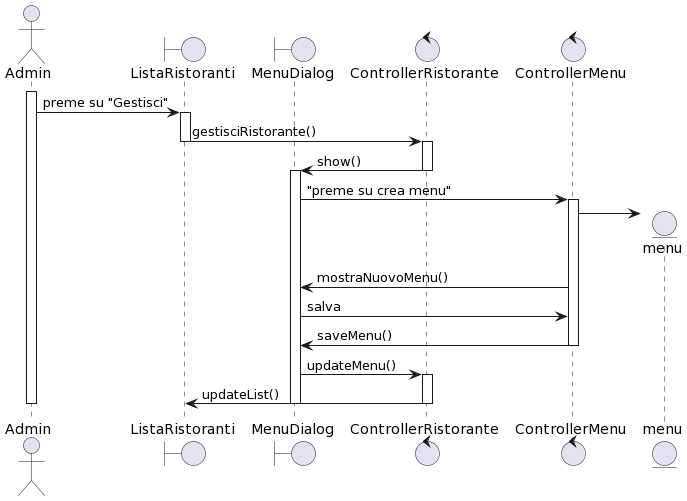
\includegraphics[scale=0.6]{assets/diagrammi/Sequence di analisi/sequence_add_menu.png}
        \caption{\textbf{Sequence}: Aggiungi menu}\label{fig:seq_add_menu}
    \end{figure}